% Created 2021-05-19 śro 08:57
% Intended LaTeX compiler: pdflatex
\documentclass[presentation]{beamer}
\usepackage[utf8]{inputenc}
\usepackage[T1]{fontenc}
\usepackage{graphicx}
\usepackage{grffile}
\usepackage{longtable}
\usepackage{wrapfig}
\usepackage{rotating}
\usepackage[normalem]{ulem}
\usepackage{amsmath}
\usepackage{textcomp}
\usepackage{amssymb}
\usepackage{capt-of}
\usepackage{hyperref}
\usepackage{minted}
\usetheme{Dresden}
\usecolortheme{sidebartab}
\usefonttheme{}
\useinnertheme{}
\useoutertheme{}
\author{Patryk Kaniewski, Dominik Gandziarek, Jakub Caban}
\date{2021-05-19}
\title{Projekt sieci i systemów korporacyjnej firmy telemarketingowej}

\hypersetup{
 pdfauthor={Patryk Kaniewski, Dominik Gandziarek, Jakub Caban},
 pdftitle={Projekt sieci i systemów korporacyjnej firmy telemarketingowej},
 pdfkeywords={},
 pdfsubject={test},
 pdfcreator={PUSB Skierniewice}, 
 pdflang={Polish}}
\begin{document}

\maketitle

\section{Wstęp}
\label{sec:orgb2a9c52}
\begin{frame}[label={sec:org7be6485}]{Wymagania Funkcjonalne}
\begin{block}{Ogólne}
\begin{itemize}
\item Dostępność sieci w każdym pomieszczeniu firmy
\begin{itemize}
\item sieć kablowa dla każdego stanowiska
\item sieć bezprzewodowa na sali konferencyjnej
\item sieć bezprzewodowa dla gosci (konferencja)
\end{itemize}
\item Wysoka dostępność systemów
\item Zapewnienie redundantnej komunikacji miedzy gałęziami sieci
\item Możliwość zarządzania usługami dostarczonymi za pomoca technologii docker
\begin{itemize}
\item uruchomienie app1 + db1
\end{itemize}
\item Mozliwosc zarzadzania usługami dostarczonymi za pomoca wirtualizacji
\begin{itemize}
\item uruchomienie app2 + db2
\end{itemize}
\end{itemize}
\end{block}
\end{frame}
\begin{frame}[label={sec:org61aabae}]{Wymagania Funkcjonalne (kont.)}
\begin{block}{Monitoring sieci}
\begin{itemize}
\item Administrator ma dostęp do statystyk użytkowania systemów
\item Administrator dostaje automatyczne powiadomienia przy dużych zmianiach w pracy
\end{itemize}
\end{block}
\begin{block}{Autoryzacja na poziomie sieci}
\begin{itemize}
\item użytkownik siadając do jakiegokolwiek biurka loguje się do sieci
\item ograniczenie dostępu do czesci sieci nieuprawnionym uzytkownikom (zarzad, pracownik, administrator, gosc konferencyjny
\end{itemize}
\end{block}
\end{frame}
\begin{frame}[label={sec:orga14ab3d}]{Wymagania Funkcjonalne (kont.)}
\begin{block}{DHCP}
\begin{itemize}
\item usługa musi być redundantna
\item jeśli jeden serwer DHCP ulegnie awarii, drugi serwer zast�pczy przejmuje jego zadania
\item Adresy IP musz� być rozdzielane z określonej puli adresów.
\item Serwer zastępczy (slave) nasłuchuje na odpowiedwnim interfejsie sieciowym, je�li nie otrzymuje odpowiedzi
\item od serwera podstawowego (master) zaczyna rozdawać hostom adresy.
\end{itemize}
\end{block}
\begin{block}{DNS}
\begin{itemize}
\item usługa musi umo�liwia� translacje nazw domenowych na adresy IP jak i odwrotnie (strefy wyszukiwania wstecz i do przodu);
\item użytkownik, kt�ry siada do swojego stanowiska musi mieć umożliwione połaczenie ze stronami internetowymi
\item zarówno poprzez adresy IP jak i nazwy domenowe;
\end{itemize}
\end{block}
\end{frame}
\section{Sieć}
\label{sec:org1869b59}
\begin{frame}[label={sec:orgc63cb2c}]{Plan bundynku}
\begin{center}
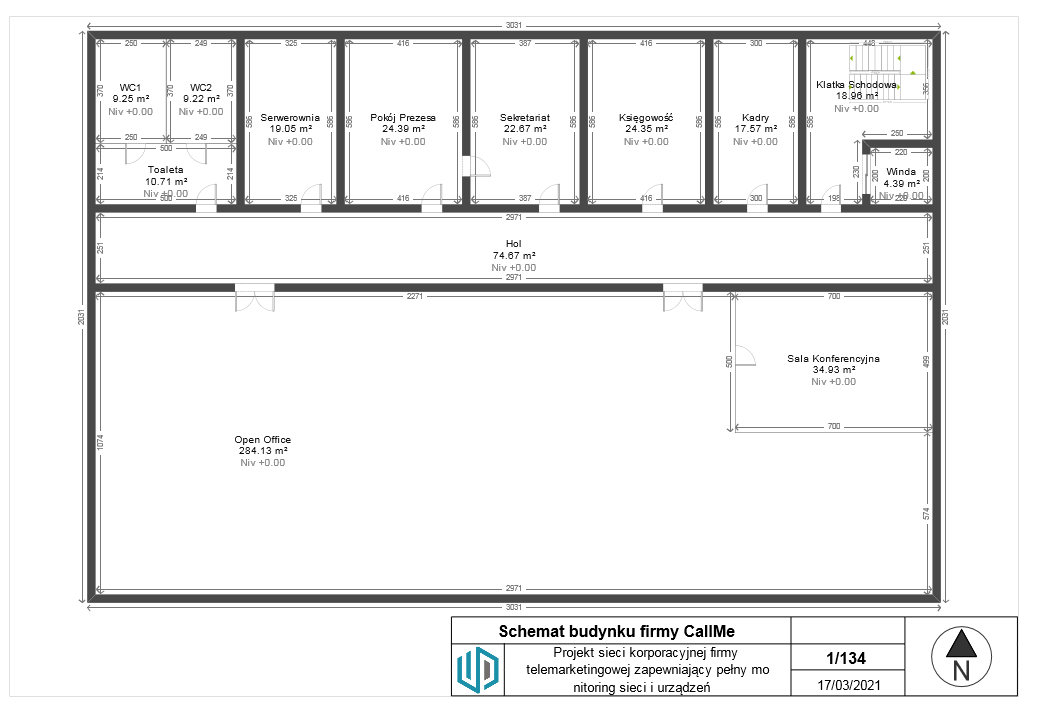
\includegraphics[width=.9\linewidth]{./data/siec/plan_budynku.png}
\end{center}
\end{frame}
\begin{frame}[label={sec:org9644cb3}]{Plan fizyczny sieci}
\begin{center}
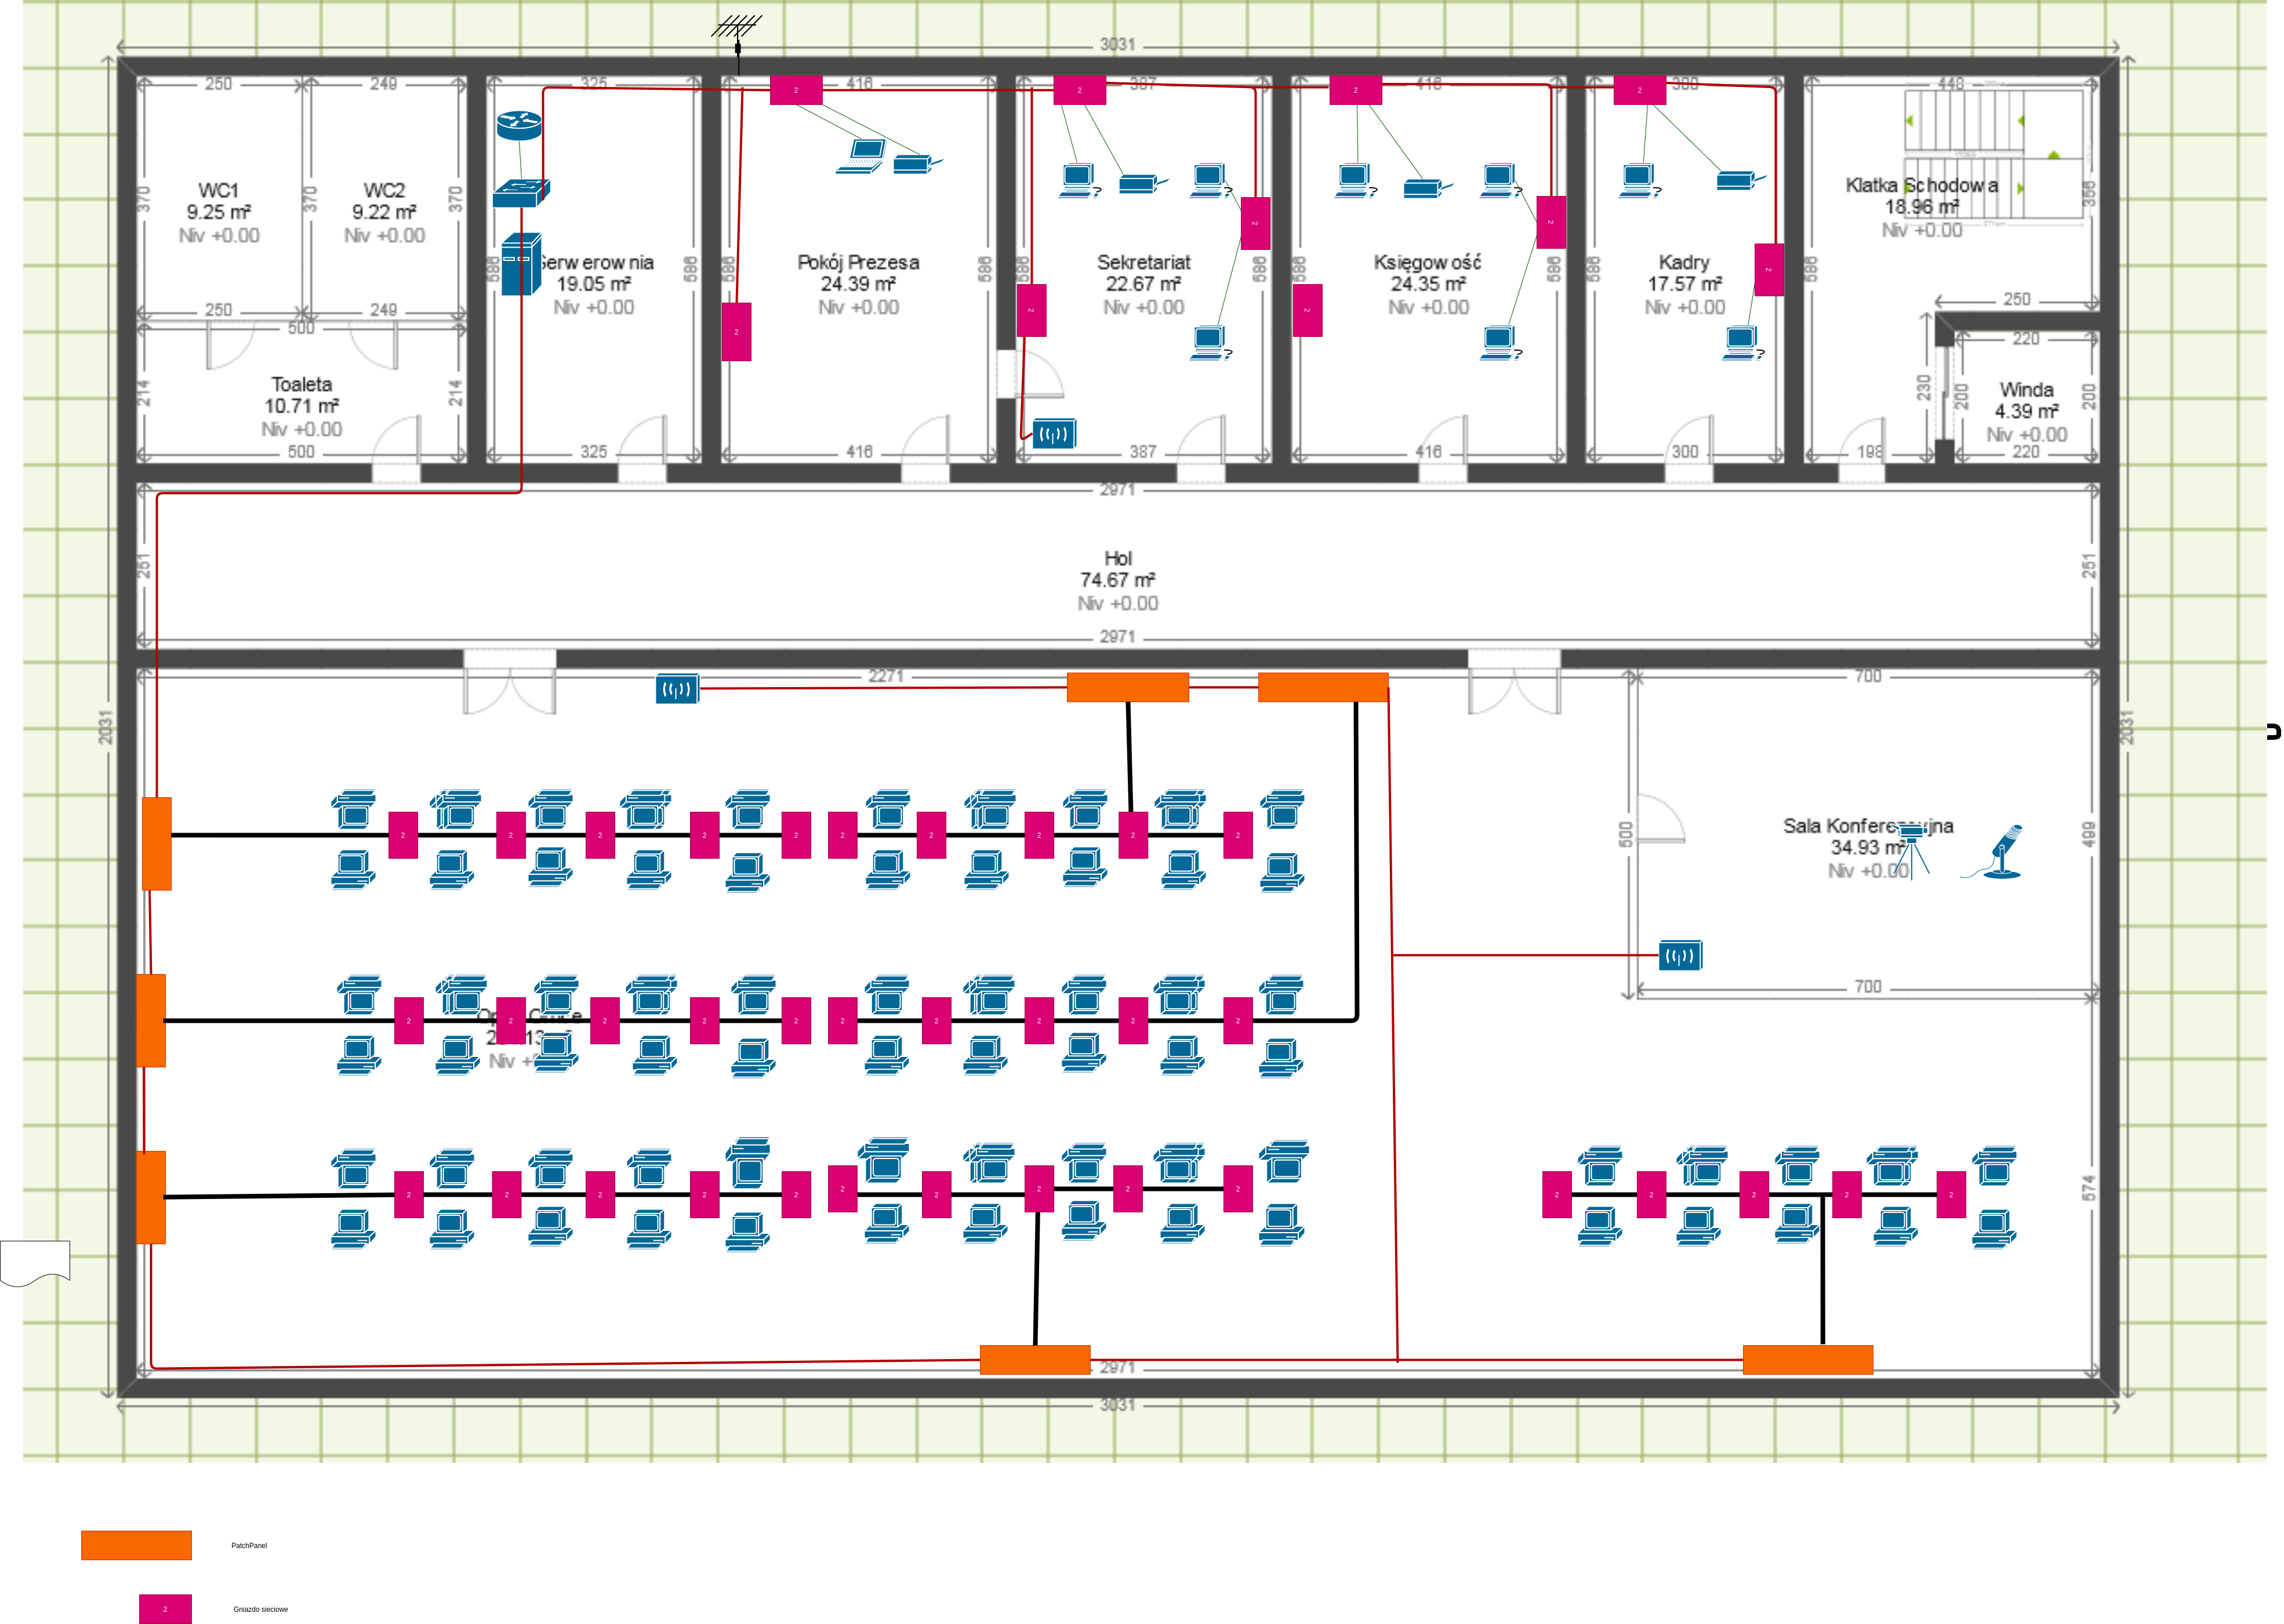
\includegraphics[width=.9\linewidth]{./data/siec/plan_fizyczny.png}
\end{center}
\end{frame}
\begin{frame}[label={sec:org67fce53}]{Plan logiczny sieci}
\begin{center}
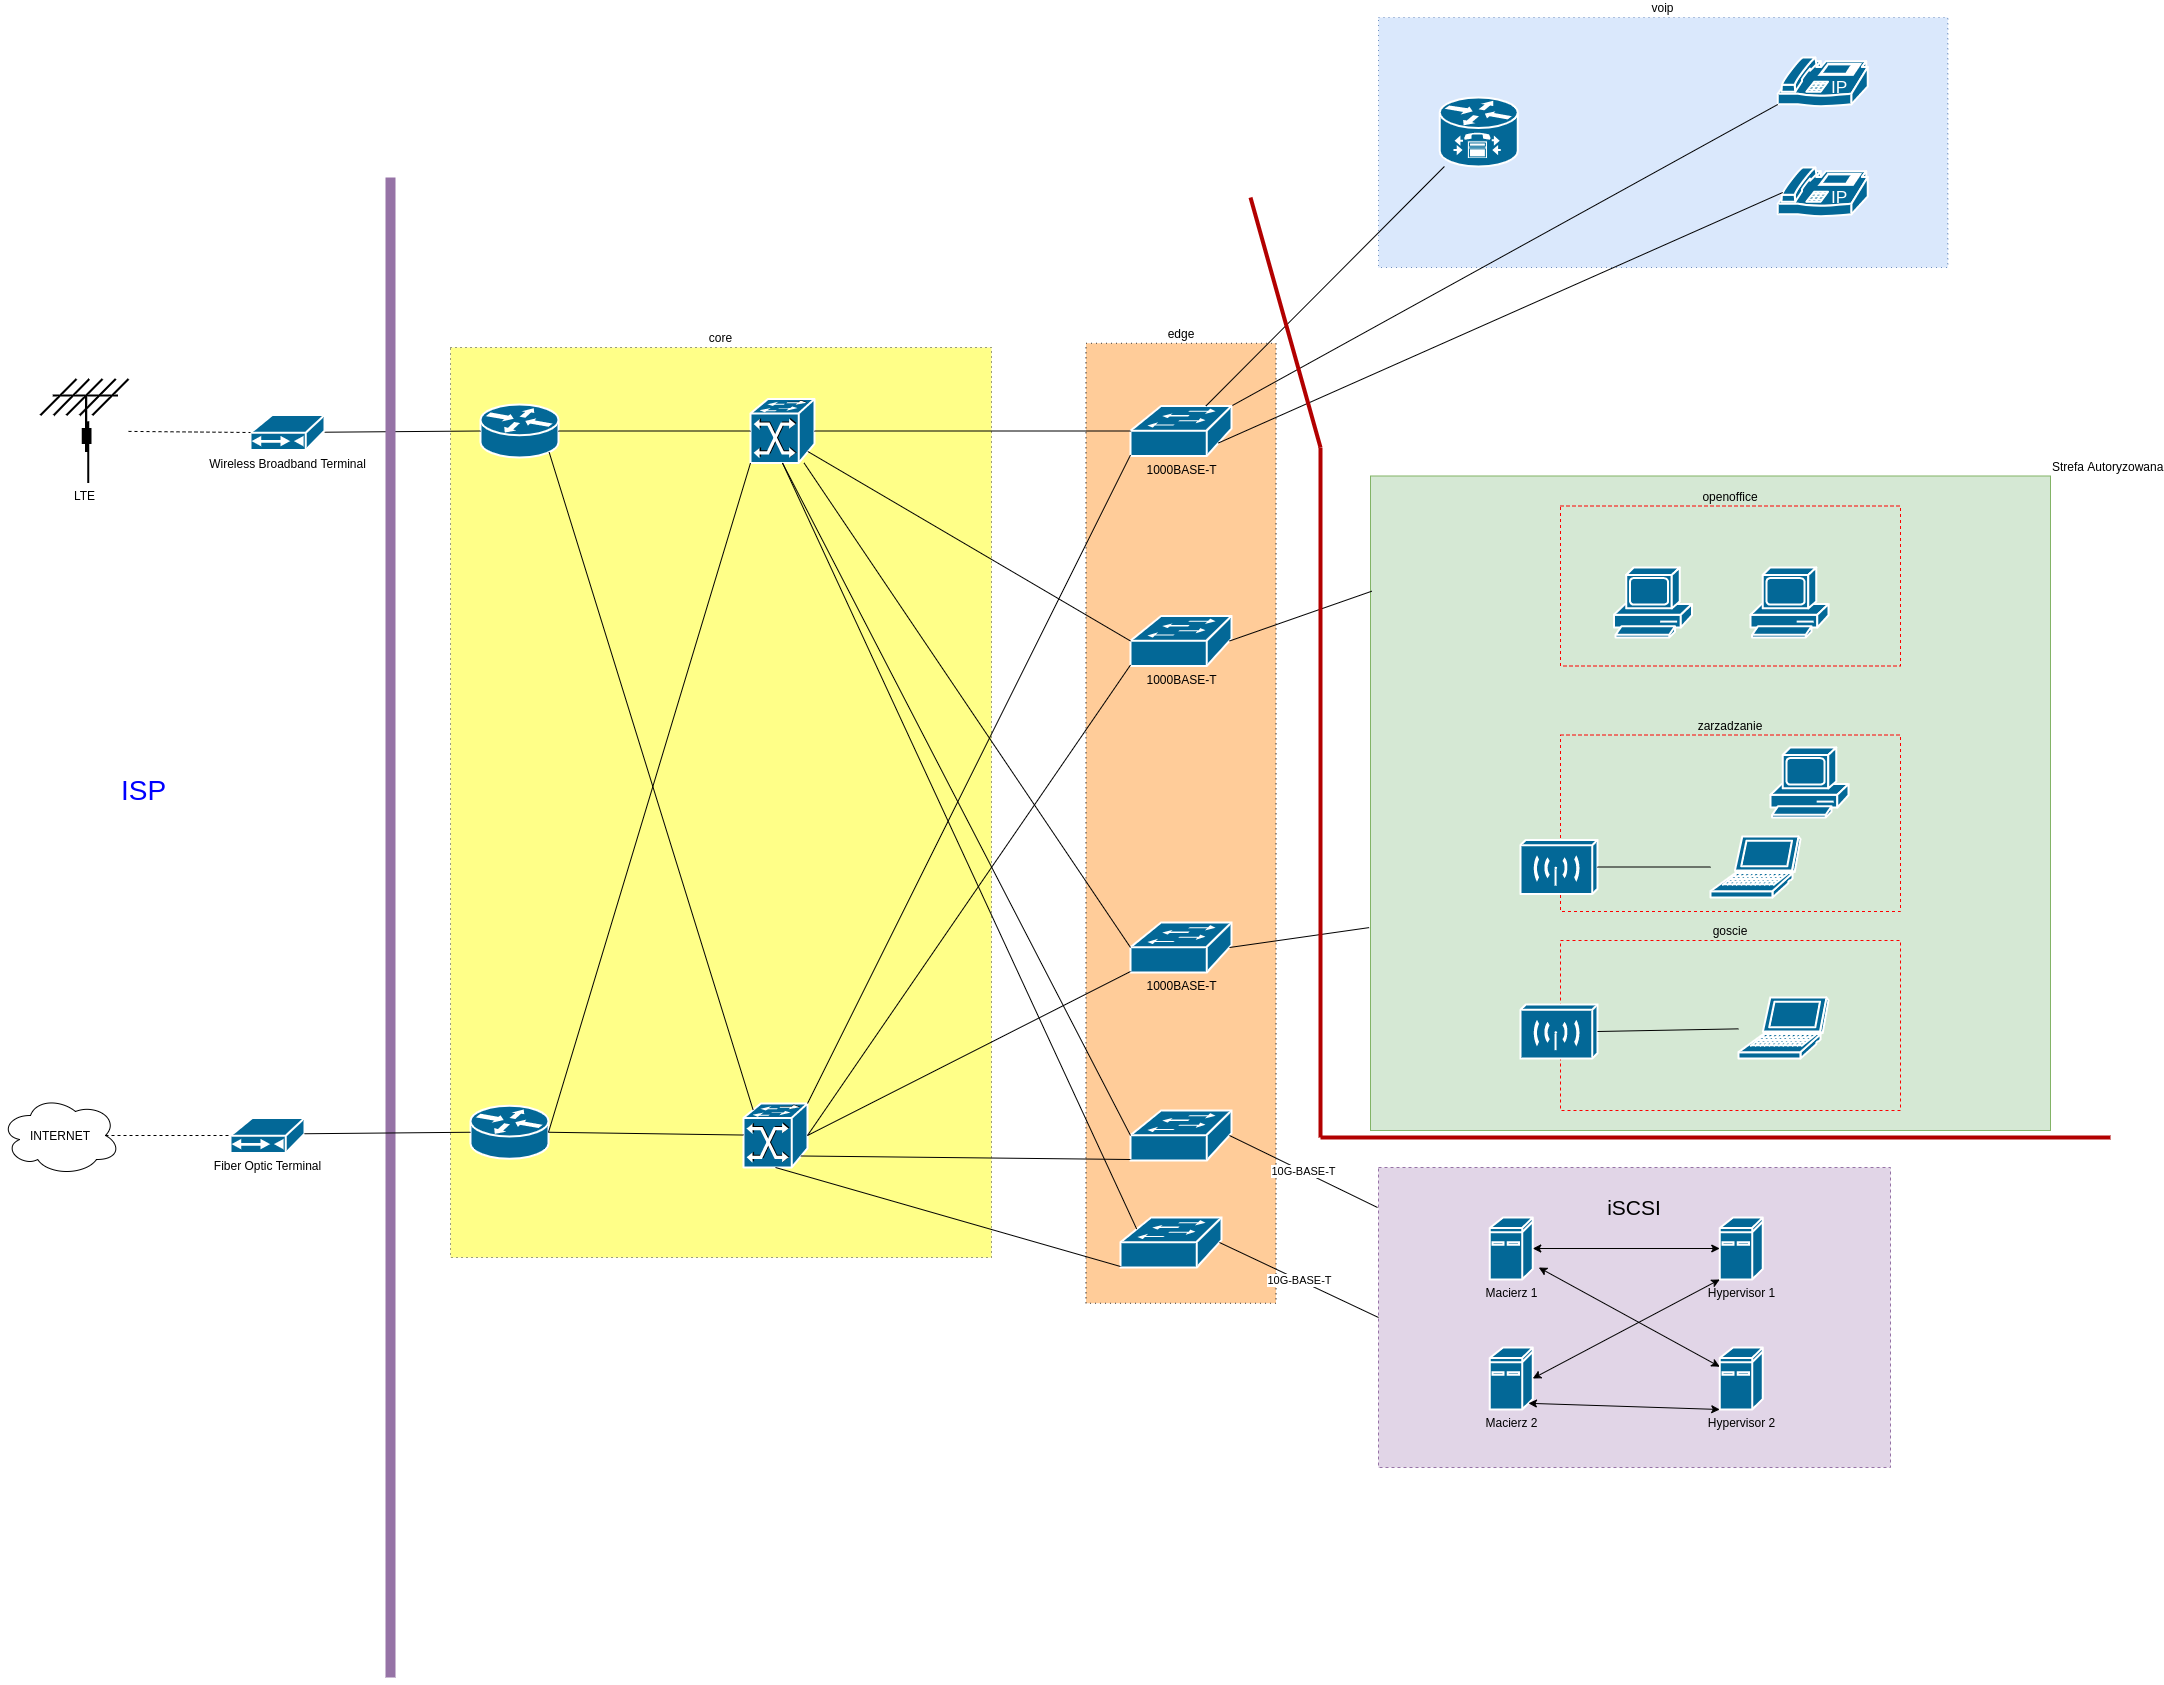
\includegraphics[width=.9\linewidth]{./data/siec/network_diagram_clean.png}
\end{center}
\end{frame}
\begin{frame}[label={sec:orgb16c778}]{Architektura serwerowa}
\begin{center}
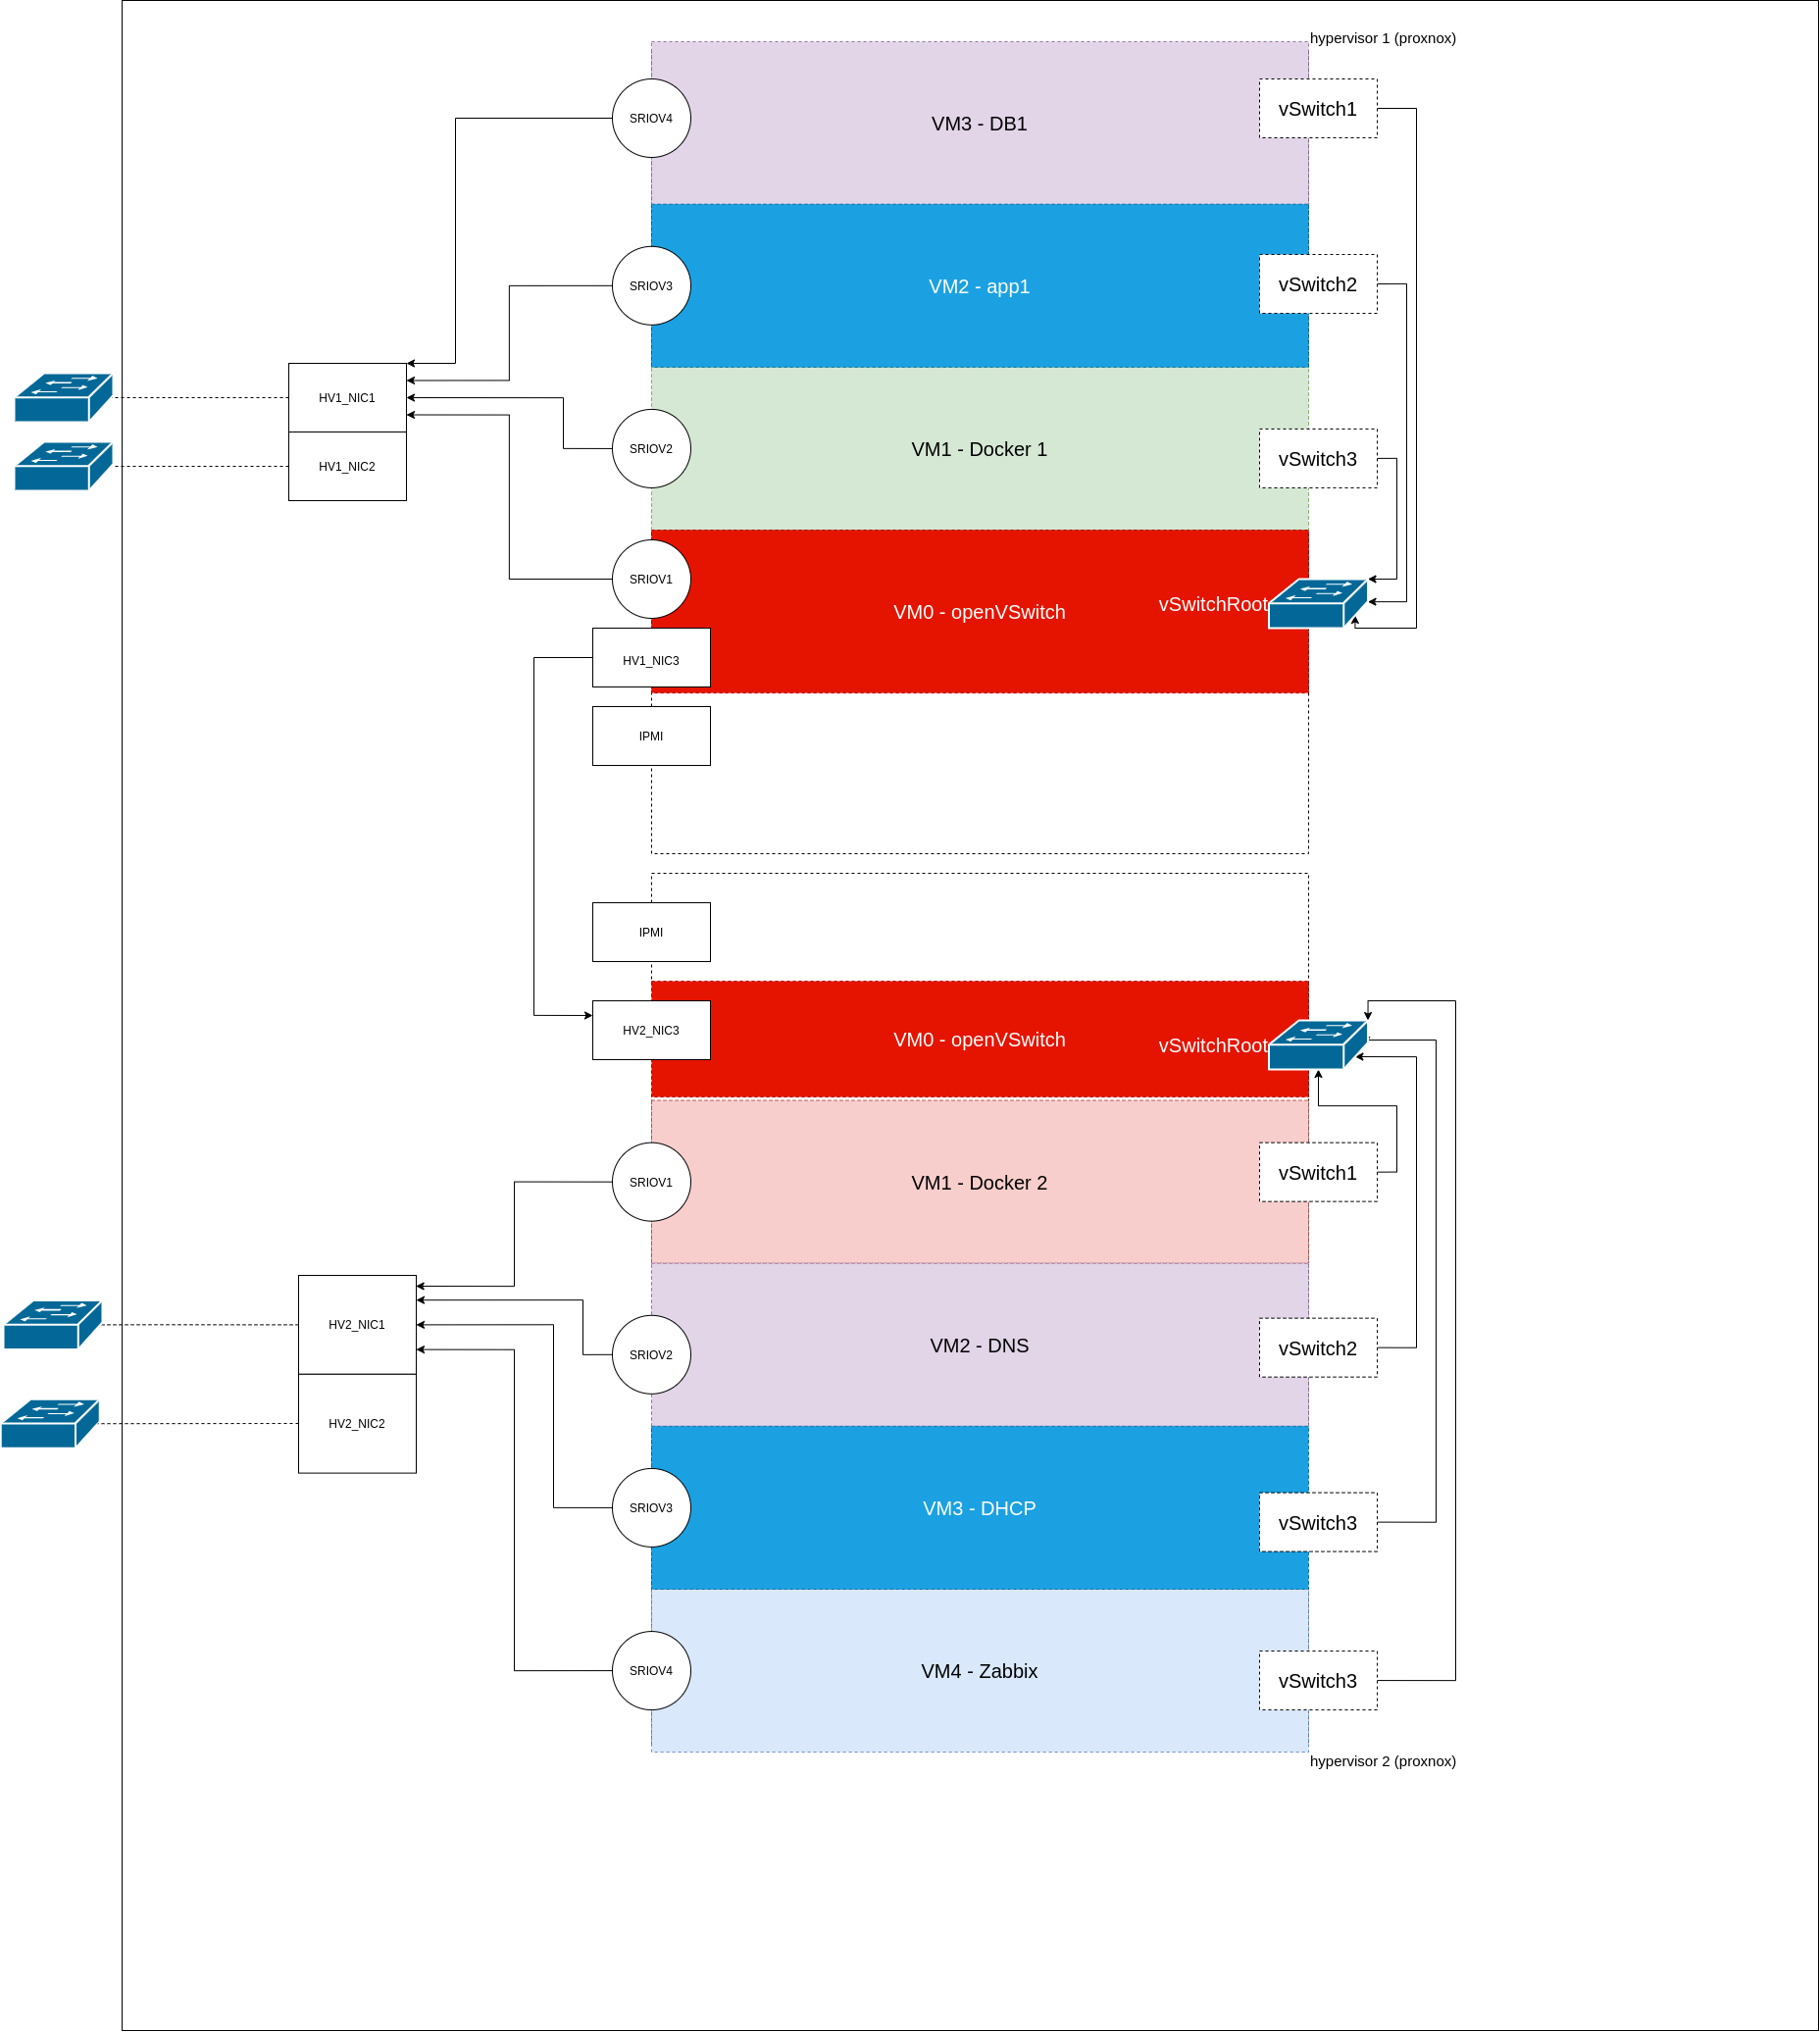
\includegraphics[width=.9\linewidth]{./data/siec/server_diagram.png}
\end{center}
\end{frame}
\section{App1/2}
\label{sec:orgb65ecbc}
\begin{frame}[label={sec:org920a3f6},fragile]{App1}
 \TINY
\begin{minted}[]{php}
<?php
$host = '192.168.200.132';
$db   = 'lab3'; $user = 'admin'; $pass = 'pwsz';
$port = '3306'; $charset = 'utf8';
$options = [
    \PDO::ATTR_ERRMODE            => \PDO::ERRMODE_EXCEPTION,
    \PDO::ATTR_DEFAULT_FETCH_MODE => \PDO::FETCH_ASSOC,
    \PDO::ATTR_EMULATE_PREPARES   => false,
];
$dsn = "mysql:host=$host;dbname=$db;charset=$charset;port=$port";
try {
     $pdo = new \PDO($dsn, $user, $pass, $options);
} catch (\PDOException $e) {
     throw new \PDOException($e->getMessage(), (int)$e->getCode());
}
$stmt = $pdo->query("SELECT * FROM aktorzy");
while ($row = $stmt->fetch()) {
    echo $row['nazwisko']."<br />\n";
}
?>
\end{minted}
\end{frame}
\begin{frame}[label={sec:org1907d78}]{App1 + db1}
\begin{center}
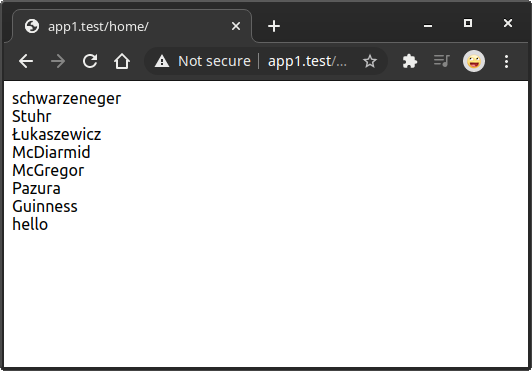
\includegraphics[width=.9\linewidth]{./data/app/app1.png}
\end{center}
\end{frame}
\begin{frame}[label={sec:orgbbcd1e8},fragile]{App2}
 \TINY
\begin{minted}[]{php}
<?php
$host = '192.168.200.145';
$db   = 'lab3'; $user = 'admin'; $pass = 'pwsz';
$port = '3306'; $charset = 'utf8';
$options = [
    \PDO::ATTR_ERRMODE            => \PDO::ERRMODE_EXCEPTION,
    \PDO::ATTR_DEFAULT_FETCH_MODE => \PDO::FETCH_ASSOC,
    \PDO::ATTR_EMULATE_PREPARES   => false,
];
$dsn = "mysql:host=$host;dbname=$db;charset=$charset;port=$port";
try {
     $pdo = new \PDO($dsn, $user, $pass, $options);
} catch (\PDOException $e) {
     throw new \PDOException($e->getMessage(), (int)$e->getCode());
}
$stmt = $pdo->query("SELECT * FROM filmy");
while ($row = $stmt->fetch()) {
    echo $row['tytul']." ".$row['rok']."<br />\n";
}
?>
\end{minted}
\end{frame}
\begin{frame}[label={sec:orgd14dd4d}]{App2 + db2}
\begin{center}
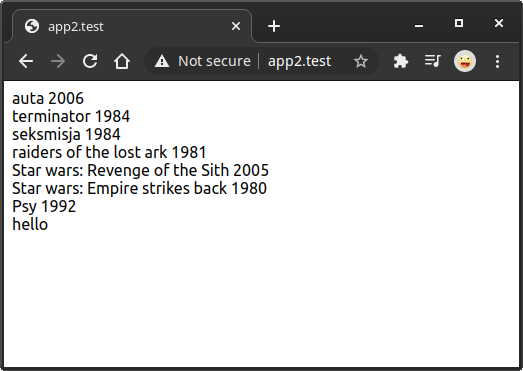
\includegraphics[width=.9\linewidth]{./data/app/app2.png}
\end{center}
\end{frame}
\section{Monitoring sieci}
\label{sec:org1c90e49}
\begin{frame}[label={sec:org98bf64b}]{Zabbix}
Zabbix jest rozwiązanie open-source (GPLv2) do monitorowania dużej ilości komponentów sieci komputerowej w tym:
\begin{itemize}
\item sieci
\item urządzeń sieciowych
\item stacji roboczych
\item serwerów
\item usług
\end{itemize}
\end{frame}
\begin{frame}[label={sec:org32ed531}]{Zabbix}
\begin{center}
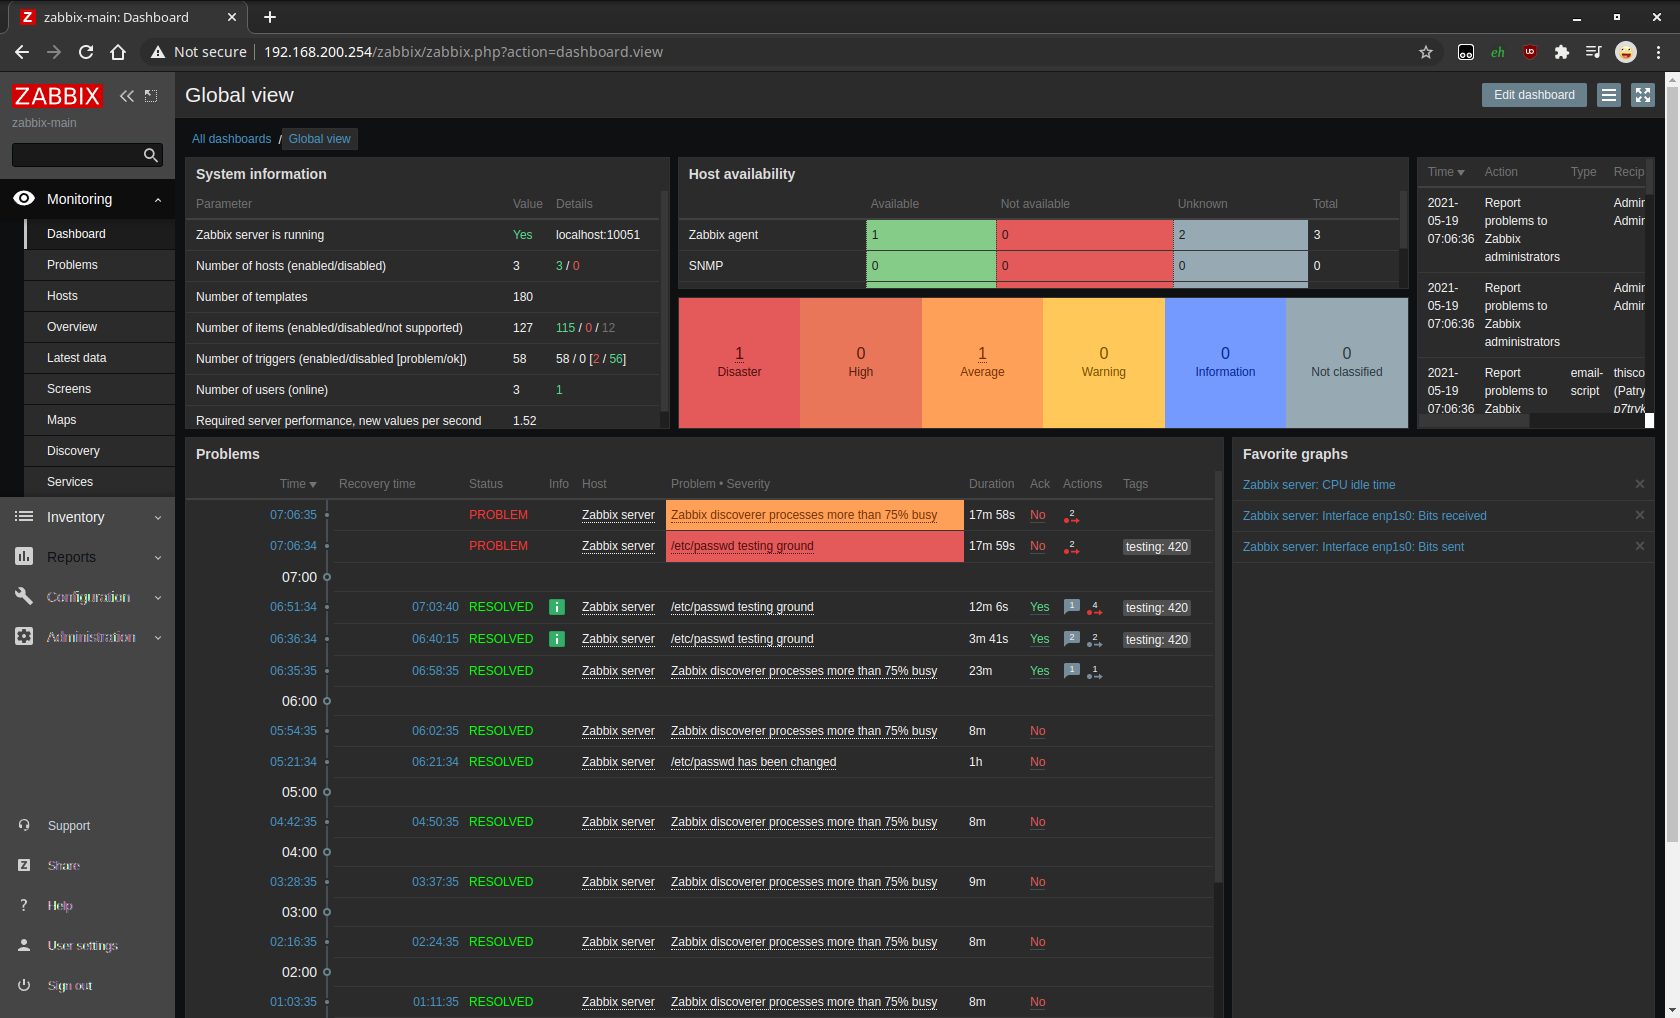
\includegraphics[width=.9\linewidth]{./data/zabbix/homepage.png}
\end{center}
\end{frame}
\begin{frame}[label={sec:org91d334f}]{Powiadomienia}
\begin{center}
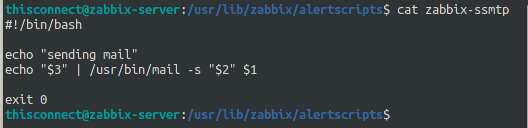
\includegraphics[width=.9\linewidth]{./data/zabbix/script.png}
\end{center}
\end{frame}
\begin{frame}[label={sec:org8f1ed0c}]{Powiadomienia (kont.)}
\begin{center}
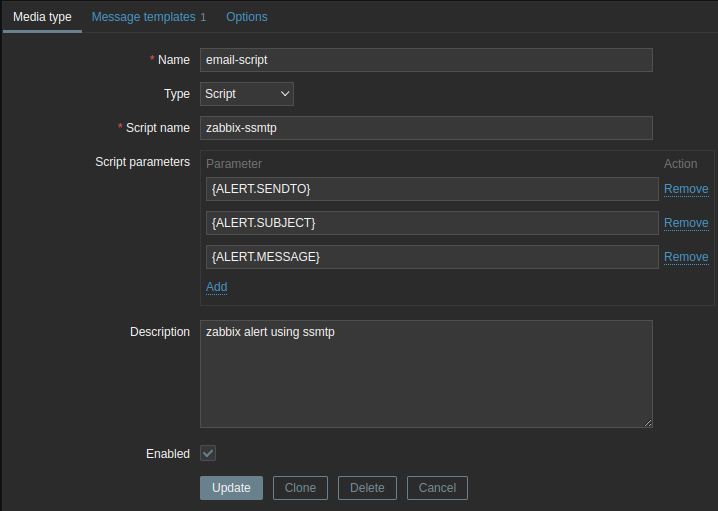
\includegraphics[width=.9\linewidth]{./data/zabbix/trigger.png}
\end{center}
\end{frame}
\section{Autoryzacja na poziomie sieci}
\label{sec:orgc76bf5d}
\begin{frame}[label={sec:orgd83ed7f}]{802.1x}
\end{frame}
\section{DHCP}
\label{sec:org3ce90e4}
\begin{frame}[label={sec:org6a731f5}]{DHCP}
\end{frame}
\section{DNS}
\label{sec:org9221f46}
\begin{frame}[label={sec:org2bda9fb}]{DNS}
\end{frame}
\end{document}
